\section{Evaluation}
In this section, we present the evaluation results of proposed SaaS and IaaS controller and their impact on cloud based application
in terms of response time and energy consumption. The goal is to advocate the benefits
and limitations of each controller while experimenting
with real cloud application and real workload traces.

\subsection{Experimental setup}
\paragraph*{\textbf{Infrastructure configuration}}The experiments were conducted in Grid'5000 Lyon site,
with 3 physical machines linked by a 10 Gbit/s Ethernet
switch and connected to wattmeter. Each machine has two
2.3GHz Xeon processors (6 cores per CPU) and 16GB of
RAM, running Linux 2.6. Openstack Liberty was used
as platform, which requires one dedicated physical machine
for the cloud controller management system. Consequently,
the other physical machines were used as compute nodes to
host VMs, which in turn, are pre-configured to run Ubuntu
12.04.

\paragraph*{\textbf{Application Configuration}} We experimented with
RUBiS application \cite{rubis}, an eBay like auction site, which
is assumed to be a representative of popular e-commerce application 
and hence interactive web application. In Brownout \cite{brownout}, authors provided a user-to-user recommendation engine that is not core functionality of service but can enhance user experience. Along with that, we implemented a fairly simple item-to-item recommendation, to offer another level of user experience. The
simple recommendation engine can be summarized as "Retrieve 10 products from same seller and same product category which has higher or same user bid count with high customer rating". The recommendation is added
to the item visualisation page and to enable it, we defined
a function that reads a file, where actuator value is updated
in each control period and execute the associated modes for
each user request. For instance, Mode 1 activates the codes of
recommendation one, mode 2 activates both recommendations
and mode 0 provides no recommendation. Furthermore, the application is deployed with all its tiers \emph{i.e.,} web and database server inside a VM using a LEMP stack\footnote{\url{https://lemp.io/}}. Each application VM and Load-balancer (LB) VM were configured with 4 cores of CPU and 8GB of memory similar to Large flavor VM. Since, we used 2 compute servers, we could use maximum of 6 VM's and minimum at 2 VM's\footnote{1 LB VM and 1 application VM}. 

\begin{figure}[h]
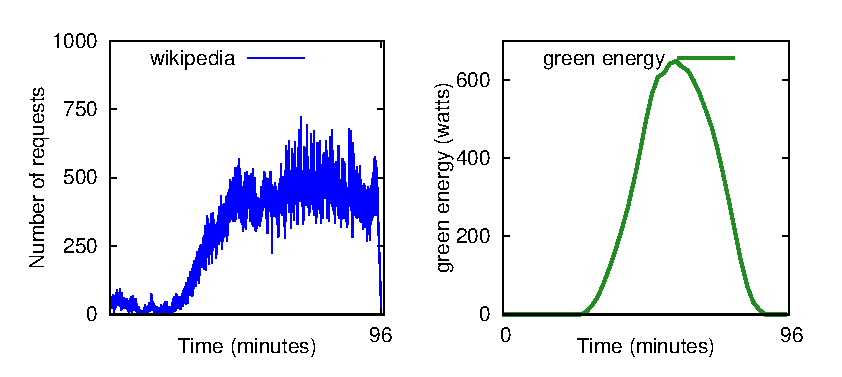
\includegraphics[width=9.0 cm, height=2.8 cm]{Graphs/workload_ucc.eps}
\caption{Workload trace}
\label{fig:workload} 
\end{figure}

\paragraph*{\textbf{Platform and Workload}} Our Proposed platform solution is hosted inside the cloud controller
machine. It monitors the 95th percentile response
time by aggregating the Nginx log of LB in each control period \emph{i.e.,} 20 seconds, whereas green energy
information is pushed by the infrastructure through an API in every 60 seconds. We took the real traffic pattern of wikipedia german page of one day [22] and scaled the data set to fit with our experiment,
which is showed at Figure 6. To generate the workload, we used Gatling as load injector and choose an
open system model, where user requests are issued without
waiting for other users response from the system. Furthermore,
we emulated read-only workload where each user arrives to the homepage, browse any item category from a
vast catalog, click on a product to extract its information,
view seller rating and his/her reputation related to the
product. Furthermore, the duration
of each experiment was 96min and each was run several
times. We considered 96min as 24 hours, i.e., each 4min in
our experiments correspond to 1 hour.


\subsection{Consideration of delaying event}

\begin{figure} [htb]
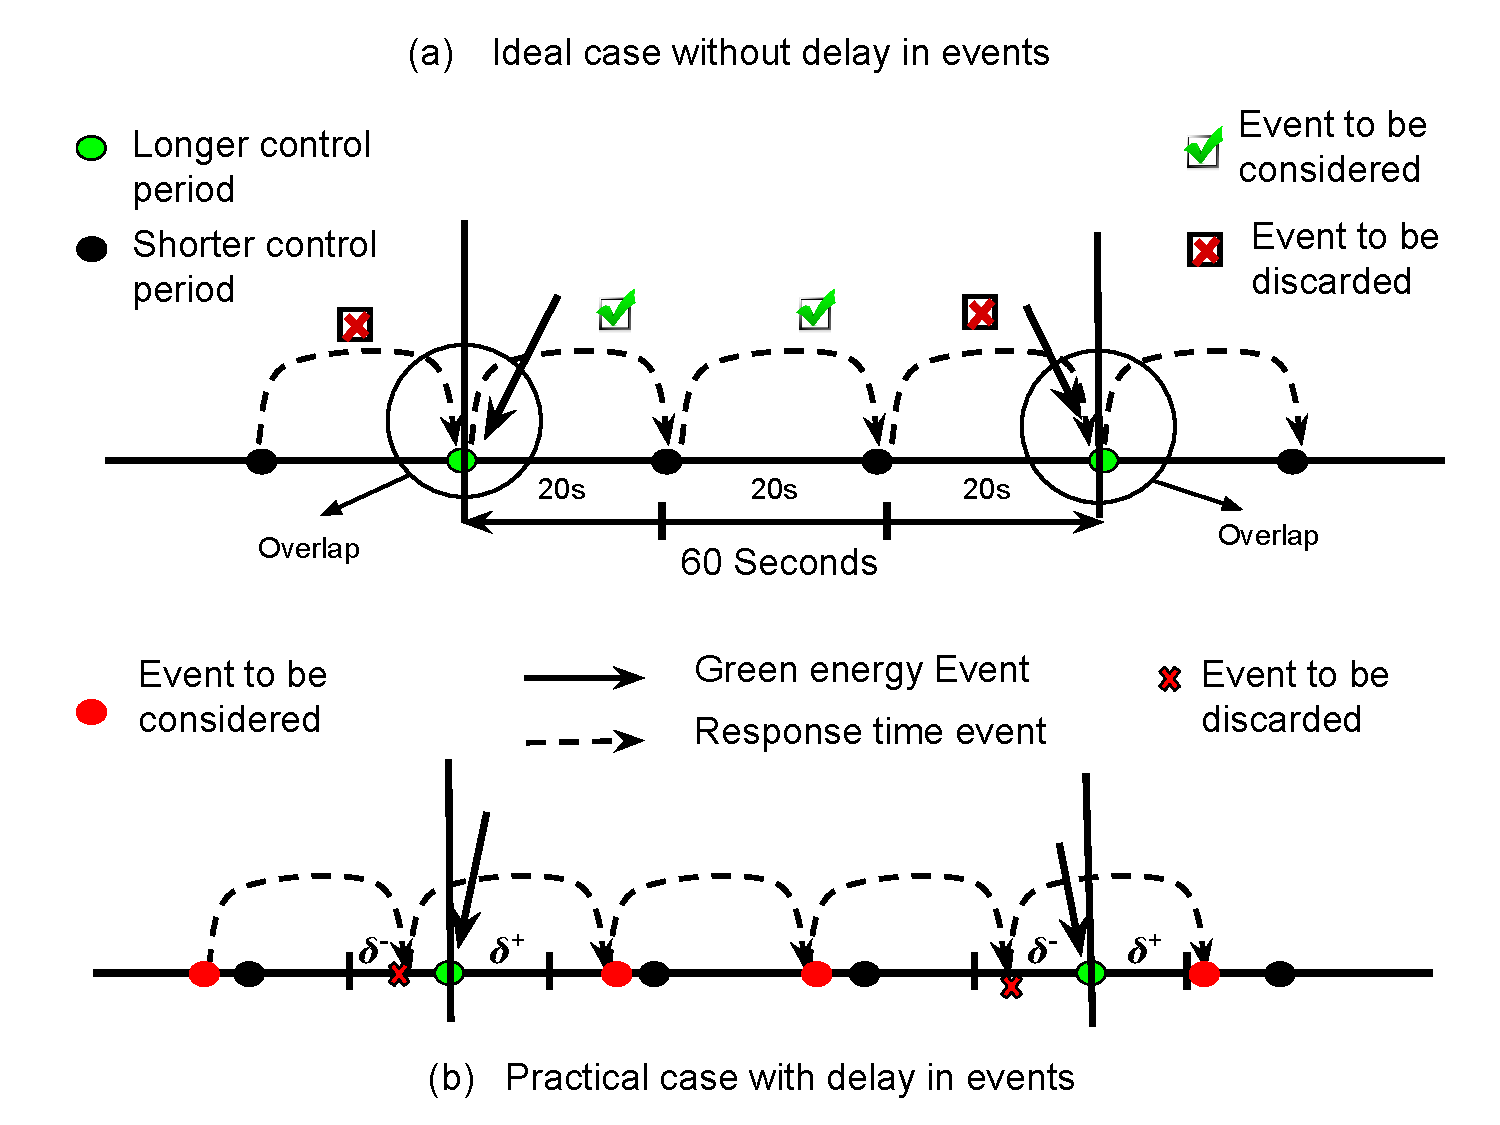
\includegraphics[scale=.35]{Graphs/implementation_UCC.pdf}
\caption{Algorithm implementation in detail}
\label{fig:implementation} 
\end{figure}

From Section \ref{saas-controller}, we see that, \emph{GE-C} controller has inner and outer loops which are activated in different time-scales and push events to the controller to make decision. In our experiments, outer (longer control period) and inner (shorter control period) loops are activated in each 60 seconds and 20 seconds respectively, which is showed in Figure \ref{fig:implementation}. Ideally, if both kind of events arrive without any delay, two different events will overlap each other. As our motivation is to maximize of green energy usage for \emph{GE-C} controller, we always make primary decision based on the green energy event pushed by IaaS by ignoring the response time event which is activated as inner loop, if both the event arrives concurrently. Concretely, it suggests that, between two big decision events in 60 seconds, we consider only two inner loop events and take actions if it is necessary indicated in Figure \ref{fig:implementation}(a).

But in case of delaying of any event, the scenario will not follow Figure \ref{fig:implementation}(a). As discussed before, the primary decision always depends on green energy event. Even though we receive response time event, no action is taken unless the system's response is high. Therefore, in case of delaying of response time event by micro to milliseconds, effects to the system remain almost unchangeable. In contrast, if the event delays by couple of seconds, for instance, inner loop event arrives just before or after the primary decision is made, it might affect the system dynamics to achieve the goal. To tackle the problem, we define a safety distance, denoted by $\delta^t$ to ensure that the controller does not take any action if response time event arrives in between "\textit{PrimaryDecision - $\delta^t$}" and "\textit{PrimaryDecision + $\delta^t$}". Figure \ref{fig:implementation}(b) illustrates the phenomena by an example. For our case, we choose safety distance as, $\delta^t$ = Time frequency of inner loop / $2$, which is equal to 10 seconds in our experiments.



\subsection{Results}

\paragraph*{\textbf{Response time}}

\begin{figure} [htb]
\centering
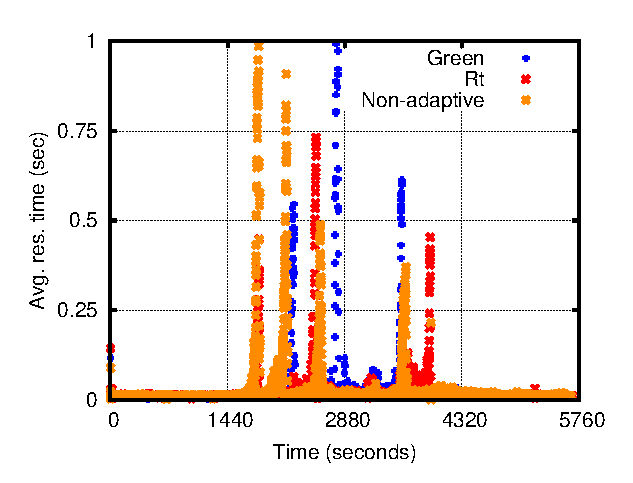
\includegraphics[scale=.8]{Graphs/response_time.eps}
\caption{Response time incurred by Controllers}
\label{fig:rt}
\end{figure}


\begin{figure} [htb]
\centering
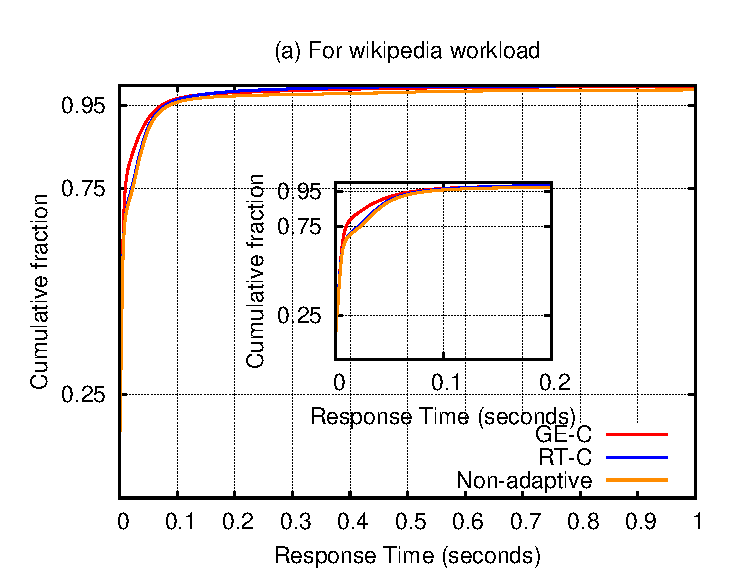
\includegraphics[scale=.75]{Graphs/percentile.eps}
\caption{Response time in percentiles}
\label{fig:perc}
\end{figure}

\paragraph*{\textbf{Energy Consumption}}

%\begin{table*}
%  \caption{Some Typical Commands}
%  \label{tab:commands}
%  \begin{tabular}{ccl}
%    \toprule
%    Command &A Number & Comments\\
%    \midrule
%    \texttt{{\char'134}author} & 100& Author \\
%    \texttt{{\char'134}table}& 300 & For tables\\
%    \texttt{{\char'134}table*}& 400& For wider tables\\
%    \bottomrule
%  \end{tabular}
%\end{table*}


%Total: 5912.49
%Green: 3395.9
%Brown: 2516.59

\begin{table*}
\caption{Energy Consumption in Watts}
  \label{tab:watt}
\begin{tabular}{cccl}
\toprule
Controller & Total Energy Consumption & Brown Energy Consumption & Green Energy Consumption\\
\midrule
Non-Adaptive & 5912.49 & 2516.59 & 3395.9 \\
RT-C & 5574.78 & 2226.16 & 3348.62  \\  %&1446.01 & 1941.32 & 3387.33 & --\\ \hline
GE-C & 4796.17 (NA > 18.88\%)(RT-C > 13.96\%) & 1632.77 (NA > 35.11\%) (RT-C > 26.65\%) & 3163.4 \textcolor{red}{(NA < 6.83\%)( RT-C < 5.53\%)} \\
\bottomrule
\end{tabular}
\end{table*}

\paragraph{\textbf{Cost analysis}}


